\documentclass{article}
\usepackage[utf8]{inputenc}
\usepackage{geometry}
 \geometry{
 a4paper,
 total={170mm,257mm},
 left=20mm,
 top=20mm,
 }
 \usepackage{graphicx}
 \usepackage{titling}

 \title{Chapter 1: Vehicle 1 - Getting Around}
\author{Fharook shaik}
\date{04 November 2024}
 
 \usepackage{fancyhdr}
\fancypagestyle{plain}{%  the preset of fancyhdr 
    \fancyhf{} % clear all header and footer fields
    \fancyfoot[R]{
\includegraphics[width=3cm]{BTULogo_englisch_grau_2x.png}}
    \fancyfoot[L]{\thedate}
    \fancyhead[L]{13869 - Braitenberg Vehikel Praktikum}
    \fancyhead[R]{\theauthor}
}
\makeatletter
\def\@maketitle{%
  \newpage
  \null
  \vskip 1em%
  \begin{center}%
  \let \footnote \thanks
    {\LARGE \@title \par}%
    \vskip 1em%
    %{\large \@date}%
  \end{center}%
  \par
  \vskip 1em}
\makeatother

\usepackage{lipsum}  
\usepackage{cmbright}

\begin{document}

\maketitle

\noindent\begin{tabular}{@{}ll}
    Student & \theauthor\\
    Professor &  Dr. Cunningham, Douglas\\
    Matrikel-Nr.: & 5014962
     
\end{tabular}

\section*{Summary}

This Chapter from \textit{Vehicles: Experiments in Synthetic Psychology} by \textit{Valentino Braitenberg} introduces the concept of creating simple and hypothetical Vehicles with basic sensory and motor functions. Braitenberg introduces \textit{Vehicle 1} (Fig. \ref{fig:vehicle-1}), the simplest possible vehicle model, with a motor and a temperature sensor. The vehicle is designed to move based on the temperature readings acquired by the sensor. The strength of the vehicle motor is directly proportional to its quality  of the sensor attached. when the temperature is too hot, the vehicle tends to move faster and slow down in cold regions.

Braitenberg draws the concept of \textit{Aristotelian Physics} on how moving objects responds to the situations they encounter. Braitenberg discussed the role of friction in shaping the vehicle 1's behavior. Friction, which resists movement, plays a critical role because it slows down the vehicle as it moves away from warmer areas, giving the appearance of thoughtful navigation. The vehicle's speed increases in warmer regions where impact of friction is reduced by the motor's stronger drive. 


% 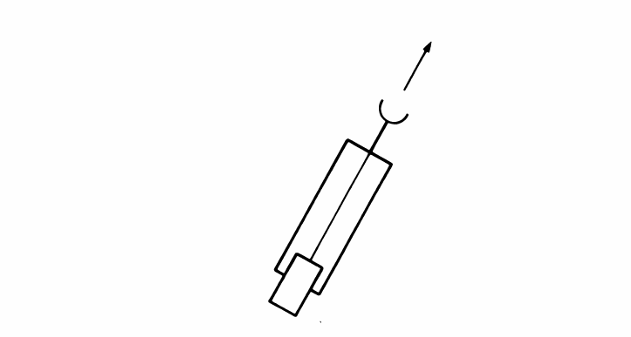
\includegraphics[scale=0.75]{Screenshot 2024-11-05 085900.png}


\begin{figure}[h]
    \centering
    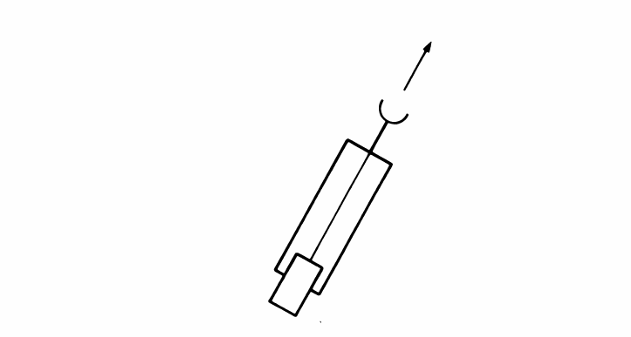
\includegraphics[scale=0.75]{Screenshot 2024-11-05 085900.png}
    \caption{Vehicle 1, Speed of the motor (Rectangular Box), Sensor (half circle at the top)}
    \label{fig:vehicle-1}
\end{figure}


In Aristotelian Physics, objects are thought to have natural tendencies. Braitenberg uses this analogy to explain vehicle 1's behavior might look purposeful (attraction to warmer areas) even though it is a simple mechanical outcome.

In conclusion, Braitenberg tells that Vehicle 1 may not posses consciousness, it is atleast alive in the sense that it shows response to its environment rather than being dead. This behavior is crucial as it shows that alive objects have some sort of intelligence, proposing that even simple machines can display life-like behaviors.

% \lipsum[1-2]

% \section*{Objectives}
% \lipsum[3-3]

% \section*{Plan}
% \lipsum[4-4]



\end{document}
